\documentclass[9pt,a4paper,twocolumn]{article}

\usepackage{amsmath}
\usepackage[a4paper,margin=15mm,columnsep=6mm]{geometry}
\usepackage{booktabs}
\usepackage{enumitem}
\usepackage{graphicx}
\usepackage[hidelinks]{hyperref}
\usepackage{microtype}
\usepackage{tabularx}
\usepackage{xcolor}

\setlength{\parindent}{0pt}
\setlength{\parskip}{3pt}
\setlist{nosep,leftmargin=*}
\renewcommand{\familydefault}{\sfdefault}
% Generated from measured summary.csv. Do not edit by hand.
\newif\ifresultspending
\resultspendingfalse

\newcommand{\ResultTable}{%
\begin{tabularx}{\columnwidth}{@{}lrrrr@{}}
\toprule
Method & Detect. & P95 ms & Jitter mm & Score\\
\midrule
Haar & 83.0\% & 46.2 & 10.7 & 20.0\\
MediaPipe & 100.0\% & 9.7 & 3.7 & 85.9\\
YuNet & 100.0\% & 28.2 & 8.4 & 56.3\\
\bottomrule
\end{tabularx}}

\newcommand{\SelectionStatement}{MediaPipe is selected for phases 2 and 3. It passed both predefined gates and achieved the highest weighted score (85.9/100) among the passing methods. YuNet also passed, but its worst normal-condition P95 latency was 28.2 ms versus 9.7 ms for MediaPipe, and its stationary 3D jitter was 8.4 mm versus 3.7 mm. Haar was excluded because it had sub-95\% detection in horizontal and 46.2 ms worst-case P95 latency.}


\title{Comparison of viewer-position tracking methods}
\author{Project 2.1: Parallax View Real-time Human-Computer Interface}
\date{Phase 1}

\begin{document}
\maketitle
\vspace{-1.5em}

\section{Purpose and scope}

The interface needs the viewer's position relative to the display so that the rendered viewpoint can follow lateral, vertical, and depth movement. This report therefore uses \emph{viewer-position tracking} to mean estimating the three-dimensional location of the midpoint between the viewer's eyes. It does not mean gaze tracking, which estimates where a person is looking.

The project manual requires component tests to cover functionality, failure conditions, real-time performance, and reproducibility~\cite{manual}. The comparison is limited to three methods that run from a normal webcam in Python: OpenCV Haar cascades, OpenCV YuNet, and MediaPipe Face Landmarker. Each method receives the same decoded video frames and produces the same output representation: two eye centres, their midpoint, and an approximate 3D position.

\section{Considered components}

\subsection{OpenCV Haar cascades}

The baseline uses OpenCV's frontal-face cascade, followed by its eye cascade within the upper part of the largest detected face. Haar cascades use hand-designed image features and a boosted cascade classifier~\cite{violaJones,opencvCascade}. The two small XML files come from OpenCV's repository; the setup command downloads explicit copies and records their checksums instead of relying on wheel package data. The method can return several eye-like regions, so the implementation selects the pair with strong horizontal separation and limited vertical difference. This simple pipeline is useful as a speed and implementation-cost baseline. Its expected weaknesses are changes in illumination, head rotation, partial occlusion, and false eye detections from glasses or eyebrows.

\subsection{OpenCV YuNet}

YuNet is a compact neural face detector. OpenCV's \texttt{FaceDetectorYN} output contains a face box, confidence score, and five landmarks, including both eyes~\cite{yunet,opencvYuNet}. This removes the second eye-detection stage used by the Haar baseline. The method has fewer facial landmarks than MediaPipe, but its output maps directly to the eye-midpoint representation and uses only the OpenCV dependency. It remains a face detector rather than a dedicated iris tracker, so the eye coordinates are coarse landmarks.

\subsection{MediaPipe Face Landmarker}

MediaPipe Face Landmarker returns a 478-point face mesh that includes iris landmarks~\cite{mediapipeGuide,mediapipeModel}. Its video mode tracks a detected face between frames instead of running the full detection pipeline for every frame. This may reduce latency and jitter, although that claim must be tested on the reference machine. The dense output also supports later head-pose work. Costs include a second runtime dependency, a larger external model bundle, and more integration code. The current 1.0.1 wheel aborted during initialisation on the reference Mac. The experiment therefore pins the official 0.10.21 Python 3.12 wheel, which passed the same model smoke test. This version constraint is part of the tested component, not an unreported setup change.

\section{Criteria and selection rule}

Table~\ref{tab:criteria} fixes the criteria before measurement. Detection success and latency receive the highest weights because a missing or late position update directly breaks the relation between head movement and the rendered view.

\begin{table}[h]
\centering
\caption{Selection criteria fixed before testing.}
\label{tab:criteria}
\begin{tabularx}{\columnwidth}{@{}XrX@{}}
\toprule
Criterion & Weight & Measure\\
\midrule
Detection success & 30\% & Frames containing a valid eye pair\\
Tracking latency & 25\% & Median and 95th percentile per-frame time\\
Stationary jitter & 20\% & Standard deviation of estimated $x$, $y$, and $z$\\
Positional error & 15\% & Euclidean error at measured reference positions\\
Robustness & 5\% & Performance loss across adverse conditions\\
Implementation cost & 5\% & Dependencies, model setup, and failure handling\\
\bottomrule
\end{tabularx}
\end{table}

A component passes the real-time gate when its 95th-percentile processing latency is below 33.3~ms, the frame budget at 30~Hz. It passes the functional gate when detection success is at least 95\% in the stationary, horizontal-motion, and distance conditions. A failed gate excludes a method from selection. Among remaining methods, each quantitative criterion is converted to a 0--100 score relative to the best and worst measured value, with higher detection success and lower latency, jitter, and error preferred. The weighted total determines the selection. Robustness is the mean detection-success retention across adverse conditions. Implementation cost uses a documented three-level rubric: 100 for OpenCV-only with two small cascade files, 50 for one external neural model, and 0 for an additional runtime plus model. Quantitative results override convenience.

\section{Experimental method}

\subsection{Reference system and controlled inputs}

Tests run on a 13-inch 2020 MacBook Pro with an Apple M1 processor, eight-core integrated GPU, 16~GB memory, macOS 26.5.2, and its built-in 720p camera. The recorder requests 1280$\times$720 at 30~Hz. Actual capture properties are recorded because the camera backend may negotiate a different mode.

One guided 170-second recording contains all controlled inputs. Its first five seconds record the viewer sitting still at a marked distance of 600~mm and are reserved for calibration. Eight labelled 15-second segments then cover stationary seating, horizontal movement, vertical movement, distance change, low light, glasses, one-eye occlusion, and head rotation. Five- or ten-second preparation intervals appear between conditions and are excluded from analysis. Every component therefore receives identical frames, avoiding changes in participant motion or illumination between methods. Each method processes every test segment three times; calibration and preparation frames do not contribute to benchmark timing or error. Identifiable source video remains local; segment definitions, learned calibration values, per-frame CSV data, configuration, checksums, code, and plots are retained for reproduction.

\subsection{Common position estimate}

Detector output and geometric conversion are evaluated separately. No interpupillary-distance value is entered. For each component, the reserved calibration segment supplies the median detected eye separation $d_0$ at the measured reference distance $z_0$. For a later eye separation $d_p$, the similar-triangles approximation gives
\[
z=z_0\frac{d_0}{d_p},\qquad
x=\frac{(u-c_x)z}{f},\qquad
y=\frac{(v-c_y)z}{f},
\]
where $(u,v)$ is the eye midpoint, $(c_x,c_y)$ is the camera principal point, and $f$ is obtained from the configured horizontal field of view. Calibrating each component separately accounts for its particular landmark definition. The approximation assumes the eye line is nearly parallel to the image plane, so head rotation is reported as a robustness condition rather than treated as accurate depth ground truth.

\subsection{Timing and statistics}

Timing starts immediately before a tracking call and ends when it returns. Video decoding, file I/O, plotting, and rendering are excluded. Every frame, including failed detections, contributes to the latency distribution. Detection success uses all frames. The report gives medians and 95th percentiles because occasional delays matter and latency need not follow a normal distribution. Stationary jitter uses sample standard deviation only for detected frames. Raw per-frame data remains available instead of reducing results to an average frame rate.

\section{Results and component selection}

\ResultTable

\ifresultspending
\begin{center}
\fcolorbox{red!60!black}{red!5}{\parbox{0.92\columnwidth}{\textbf{Measurement status: pending.} The code and protocol are complete, but reporting values before recording the controlled inputs would fabricate evidence.}}
\end{center}
\else
\IfFileExists{figures/detection_success.pdf}{%
\begin{figure}[h]
\centering
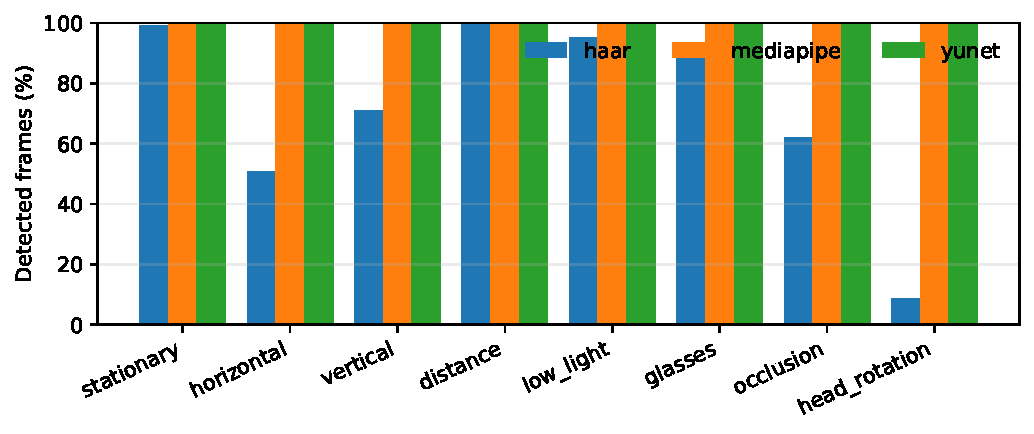
\includegraphics[width=\columnwidth]{figures/detection_success.pdf}
\caption{Detection success by test condition.}
\end{figure}}{}
\IfFileExists{figures/latency_p95.pdf}{%
\begin{figure}[h]
\centering
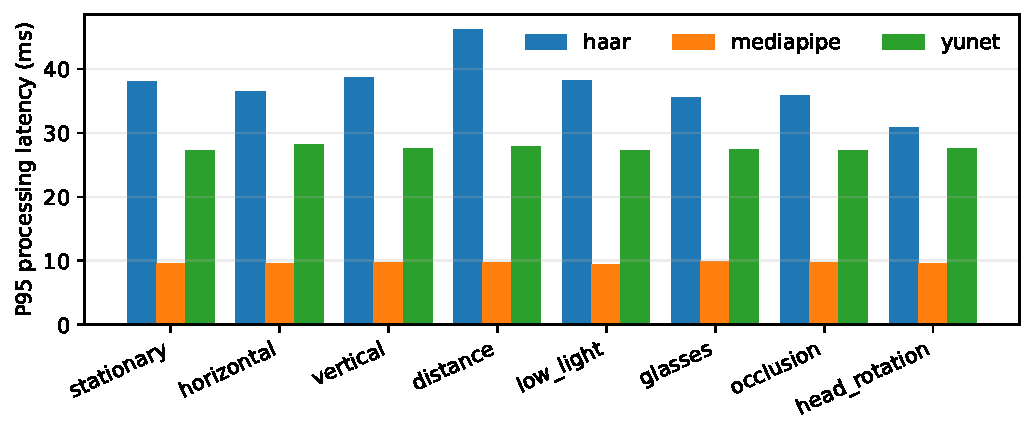
\includegraphics[width=\columnwidth]{figures/latency_p95.pdf}
\caption{95th-percentile tracking latency by condition.}
\end{figure}}{}
\fi

\SelectionStatement

The selected component will enter phase 2 behind the common tracker interface. This keeps camera capture, coordinate conversion, logging, and later parallax rendering independent from the chosen detector. Phase 2 will integrate the selected method with the renderer and measure end-to-end latency. Phase 3 will tune smoothing without hiding delay, extend adverse-condition testing, and include the tracking failures in the user-study discussion. If no method passes both gates, phase 2 will use the method with the highest detection success while testing a reduced input resolution and an asynchronous capture pipeline.

\section{Validity and reproducibility}

The test controls input frames and software settings, but it does not represent every face, skin tone, camera, or room. A single participant cannot establish population-level robustness. Approximate depth depends on the measured reference distance, stable seating during calibration, and the camera-field-of-view estimate. The final report must state these assumptions and avoid presenting the estimate as laboratory-grade eye tracking. Repository commands recreate the environment, download official models, record one guided session, isolate its configured segments, run three repetitions, and regenerate CSV files and figures without editing source code.

\begin{thebibliography}{9}\small
\bibitem{manual} Maastricht University, \emph{Project 2.1: Parallax View Real-time Human-Computer Interface, Project Manual}, 26 August 2026.
\bibitem{violaJones} P. Viola and M. Jones, ``Rapid object detection using a boosted cascade of simple features,'' CVPR, 2001.
\bibitem{opencvCascade} OpenCV, ``Cascade Classifier,'' OpenCV 4.12 documentation, \url{https://docs.opencv.org/4.12.0/db/d28/tutorial_cascade_classifier.html}.
\bibitem{yunet} W. Wu, H. Peng, and S. Yu, ``YuNet: A tiny millisecond-level face detector,'' \emph{Machine Intelligence Research}, 20(5), 2023.
\bibitem{opencvYuNet} OpenCV, ``FaceDetectorYN class reference,'' \url{https://docs.opencv.org/doc/doxygen/html/df/d20/classcv_1_1FaceDetectorYN.html}.
\bibitem{mediapipeGuide} Google, ``Face landmark detection guide for Python,'' updated 17 August 2026, \url{https://developers.google.com/edge/mediapipe/solutions/vision/face_landmarker/python}.
\bibitem{mediapipeModel} Google, ``MediaPipe Face Mesh V2 model card,'' \url{https://storage.googleapis.com/mediapipe-assets/Model%20Card%20MediaPipe%20Face%20Mesh%20V2.pdf}.
\end{thebibliography}

\end{document}
